\documentclass{article}
\usepackage[hscale=0.7,vscale=0.8]{geometry}
\usepackage{microtype}
\usepackage[utf8]{inputenc}
\usepackage[T1]{fontenc}
\usepackage{graphicx}
\usepackage{xr-hyper}
\usepackage[hidelinks]{hyperref}
\usepackage[dvipsnames]{xcolor}
\usepackage[htt]{hyphenat}
\usepackage{ellipsis}
\usepackage{amsmath}
\usepackage{amsthm}
\usepackage{amssymb}
\usepackage{mathabx}
\usepackage{algorithm}
\usepackage{algpseudocode}
\usepackage{listings}
\usepackage{authblk}
\usepackage{xr}
\externaldocument{main}
\newcommand{\todo}[1]{\textbf{\textsc{\textcolor{red}{(TODO: #1)}}}}
\lstset{breaklines=true, basicstyle=\small\ttfamily, columns=flexible}
\newcommand{\Break}{\State \textbf{break} }
\newcommand\CONDITION[2]%
  {\begin{tabular}[t]{@{}l@{}l@{}}
     #1&\\ \phantom{and} #2
   \end{tabular}%
  }
\algdef{SE}[MIF]{MultiLineIf}{MultiLineEndIf}[1]%
  {\algorithmicif\ \CONDITION{#1}{\ \algorithmicthen}}%
  {\algorithmicend\ \algorithmicif}% thanks to https://tex.stackexchange.com/a/329272
\algnewcommand{\LineComment}[1]{\(\triangleright\) #1}
\usepackage{rotating}
\usepackage{booktabs}
\usepackage{subfig}
\usepackage[font=small,labelfont=bf]{caption}
\usepackage{seqsplit}
\usepackage{multirow}
\input{ushyphex.tex}
% define new ref commands so that there isn't a wrap / page break between e.g. "Table" and "2".
\newcommand{\tabref}[1]{Table~\ref{#1}}
\newcommand{\figref}[1]{Figure~\ref{#1}}
\newcommand{\secref}[1]{Section~\ref{#1}}
\newcommand{\algoref}[1]{Algorithm~\ref{#1}}
\newcommand{\beginsupplement}{%
        \setcounter{table}{0}
        \renewcommand{\thetable}{S\arabic{table}}%
        \setcounter{figure}{0}
        \renewcommand{\thefigure}{S\arabic{figure}}%
        \setcounter{algorithm}{0}
        \renewcommand{\thealgorithm}{S\arabic{algorithm}}%
        \setcounter{section}{0}
        \renewcommand{\thesection}{S\arabic{section}}%
}
\newcommand{\code}[1]{\texttt{#1}}

\begin{document}
\beginsupplement
\title{Supplementary Materials: Progressive alignment with Cactus: a multiple-genome aligner for the thousand-genome era}
\author{}
\maketitle
%%%%%<*cactusPaperSupplement>


\begin{table}
\begin{center}
\begin{tabular}{l|l|l|l|l}
Aligner	& Alignathon entry name & Precision	& Recall	& F1 \\
\midrule
Progressive Cactus (this manuscript) & --- & 0.730	& 0.873	& 0.795 \\
Cactus (Alignathon version) & \texttt{cactus} & 0.706	& 0.885	& 0.785 \\
VISTA-LAGAN~\cite{vistaLagan} & \texttt{brudno}	& 0.619	& 0.791	& 0.694\\
EPO~\cite{enredoPecan} & \texttt{ebi.epo} &	0.224 &	0.893 &	0.359 \\
Mercator/Pecan~\cite{mercator,pecan} & \texttt{ebi.mp} &	0.368 &	0.878 &	0.519 \\
PSAR-Align~\cite{psarAlign} & \texttt{kimMa}	& 0.614	& 0.826	& 0.703 \\
AutoMZ~\cite{tba} & \texttt{minmei.automz}	& 0.606	& 0.694	& 0.647 \\
TBA~\cite{tba} & \texttt{minmei.tba}	& 0.640	& 0.769	& 0.699 \\
Mugsy~\cite{mugsy} & \texttt{mugsy}	& 0.065	& 0.931	& 0.122 \\
Robusta~\cite{robusta} & \texttt{robusta}	& 0.357	& 0.744	& 0.482 \\
GenomeMatch & \texttt{softberry.v1}	& 0.104	& 0.980	& 0.188 \\
GenomeMatch & \texttt{softberry.v2}	& 0.104	& 0.974	& 0.187 \\
GenomeMatch & \texttt{softberry.v3}	& 0.105	& 0.968	& 0.189 \\
MULTIZ~\cite{tba} & \texttt{ucsc}	& 0.616	& 0.818	& 0.703 \\
\end{tabular}
\caption{Precision, recall, and F1 scores for the simulated mammals dataset from the Alignathon~\cite{earl2014alignathon}. All alignments except for Progressive Cactus are as submitted for the Alignathon.}\label{tab:alignathonMammals}
\end{center}
\end{table}
\begin{table}
\begin{center}
\begin{tabular}{l|l|l|l|l}
Aligner	& Alignathon entry name & Precision	& Recall	& F1 \\
\midrule
Progressive Cactus (this manuscript)	& --- & 0.986	& 0.991	& 0.989 \\
Cactus (Alignathon version)	& \texttt{cactus} & 0.984	& 0.983	& 0.983 \\
VISTA-LAGAN~\cite{vistaLagan} & \texttt{brudno}	& 0.978	& 0.983	& 0.980 \\
Mercator/Pecan~\cite{mercator,pecan} & \texttt{compara}	& 0.940 &	0.996 &	0.967 \\
PSAR-Align~\cite{psarAlign} & \texttt{kimMa}	& 0.980	& 0.995	& 0.988 \\
AutoMZ~\cite{tba} & \texttt{minmei.automz}	& 0.980	& 0.992	& 0.986 \\
TBA~\cite{tba} & \texttt{minmei.tba}	& 0.981	& 0.992	& 0.986 \\
Mugsy~\cite{mugsy} & \texttt{mugsy}	& 0.978	& 0.996	& 0.987 \\
progressiveMauve~\cite{progressiveMauve} & \texttt{pmauve} & 0.971 & 0.997 &	0.984 \\
Robusta~\cite{robusta} & \texttt{robusta}	& 0.941	& 0.986	& 0.963 \\
GenomeMatch & \texttt{softberry.v1}	& 0.898	& 0.997	& 0.945 \\
GenomeMatch & \texttt{softberry.v2}	& 0.898	& 0.972	& 0.934 \\
GenomeMatch & \texttt{softberry.v3}	& 0.905	& 0.261	& 0.405 \\
MULTIZ~\cite{tba} & \texttt{ucsc}	& 0.980	& 0.992	& 0.986 \\
\end{tabular}
\caption{Precision, recall, and F1 scores for the simulated primates dataset from the Alignathon~\cite{earl2014alignathon}.}\label{tab:alignathonPrimates}
\end{center}
\end{table}

\begin{table}
\begin{center}
    \begin{tabular}{l|l|r|r|l|r|r}
    \multirow{2}{*}{Species}	& \multicolumn{3}{c}{Low-quality assembly alignment} & \multicolumn{3}{c}{High-quality assembly alignment} \\
    \cmidrule{2-4} \cmidrule{5-7}
    & Assembly & Scaffold N50 & Contig N50 & Assembly &	Scaffold N50 & Contig N50 \\
    \midrule
Gorilla	& gorGor3 & 913,958&	11,691&	Susie3&	20,634,945&	9,406,846 \\
Mouse lemur&	micMur1&	140,884&	3,511&	Mmur\_3.0&	108,171,978&	210,702 \\
Chinese hamster&	criGri1&	1,558,295&	27,129&	criGriCHOV2&	62,039,716&	97,133 \\
Pig&	susScr3&	576,008&	69,503&	susScr11&	88,231,837&	48,231,277 \\
Horse&	equCab2&	46,749,900&	112,381&	equCab3&	87,230,776&	1,502,753 \\
Rhesus&	rheMac8&	4,193,270&	107,172&	rheMac10&	82,346,004& 	46,608,966 \\
Camel&	ASM164081v1&	31,503&	31,503&	CamDro3&	70,369,702&	236,391 \\
\end{tabular}
\caption{Assembly versions used in the alignments of low-quality and high-quality assemblies. In addition to these 7 genomes, 4 others were included in each alignment with the same assemblies in both: human (GRCh38), mouse (mm10), rat (rn6), and dog (canFam3).}\label{tab:assembly_quality_comparison_assemblies}
\end{center}
\end{table}

\begin{table}[ht]
\centering
\begin{tabular}{l|r|r}
\multirow{2}{*}{Genome} & \multicolumn{2}{c}{Coverage on the human genome} \\
\cmidrule{2-3}
 & Alignment of high-quality assemblies & Alignment of low-quality assemblies \\ 
\midrule
Human & 1.00 & 1.00 \\ 
Gorilla & 0.90 & 0.85 \\ 
Rhesus & 0.83 & 0.82 \\ 
Mouse lemur & 0.54 & 0.43 \\
Horse & 0.51 & 0.50 \\ 
Dog & 0.47 & 0.47 \\ 
Pig & 0.46 & 0.42 \\ 
Camel & 0.46 & 0.46 \\ 
Chinese hamster & 0.34 & 0.33 \\ 
Mouse & 0.33 & 0.32 \\ 
Rat & 0.33 & 0.32 \\ 
\end{tabular}
\caption{Coverage on the human genome in the high-quality vs. low-quality assembly alignments.}\label{tab:new_vs_old_assemblies_coverage}
\end{table}

\begin{figure}
\begin{center}
\subfloat[Jarvis]{\includegraphics[width=0.5\textwidth]{jarvis14}}
\subfloat[Prum]{\includegraphics[width=0.5\textwidth]{prum15}} \\
\subfloat[Consensus]{\includegraphics[width=0.5\textwidth]{consensus}}
\subfloat[Permuted]{\includegraphics[width=0.5\textwidth]{permute}}
\caption[Guide trees used in the guide-tree influence analysis]{Guide trees used in the guide-tree influence analysis.}\label{fig:guideTreeTrees}
\end{center}
\end{figure}

\begin{figure}
\begin{center}
\includegraphics[width=\textwidth]{jarvis_prum_compare_matrix}
\caption{Species-by-species breakdown of similarity between the alignments with guide-trees based on Jarvis and Prum. Similarity for every cell of the matrix is based on F1 score for pairs of aligned bases found to be shared or unshared between the two alignments.}\label{fig:jarvisPrumCompareMatrix}
\end{center}
\end{figure}

\begin{figure}
\begin{center}
\includegraphics[width=\textwidth]{jarvis_prum_compare}
\caption{Comparison between Jarvis (left) and Prum (right) topologies (branch lengths not to scale), with branches above clades not shared between the two topologies highlighted in red.}\label{fig:jarvisPrumCompare}
\end{center}
\end{figure}

\begin{table}
\begin{center}
\begin{tabular}{lllll}
\toprule
\multirow{2}{*}{Genome} & \multicolumn{2}{c}{Coding genes missing from final set} & \multicolumn{2}{c}{Coding transcripts missing from final set} \\
\cmidrule{2-3} \cmidrule{4-5}
& Outgroup filtering & Best-hit filtering & Outgroup filtering & Best-hit filtering \\
\midrule
Chimpanzee & 1716 & 1612 & 6244 & 5872 \\
Gorilla & 1829 & 1647 & 6469 & 6100 \\
\bottomrule
\end{tabular}
\caption[Genes / transcripts missing in the ``consensus'' CAT gene set in the paralogy-filtering comparison]{Number of human genes / transcripts that have no assigned ortholog in the ``consensus'' CAT gene set across the different alignments.}\label{tab:mapqCat}
\end{center}
\end{table}

\begin{table}
\begin{center}
\begin{tabular}{lll}
\toprule
\multirow{2}{*}{Genome} & \multicolumn{2}{c}{Transcript projections filtered during initial pass} \\
\cmidrule{2-3}
& Chimpanzee & Gorilla  \\
\midrule
Outgroup filtering & 43709 & 31678\\
Best-hit filtering & 13567 & 15765\\
\bottomrule
\end{tabular}
\caption[Number of transcripts filtered in initial step of CAT]{Number of transcripts filtered out in the initial \texttt{pslCDnaFilter} step of CAT, which attempts to remove paralogs and processed pseudogenes.}\label{tab:mapqCatCDNAFilter}
\end{center}
\end{table}

\begin{table}
\begin{center}
\begin{tabular}{l|l}
Alignment & URL\\
\hline
Jarvis & \url{https://s3.amazonaws.com/alignment-output/cactus48BIRDS_jarvis14.hal} \\
Prum & \url{https://s3.amazonaws.com/alignment-output/cactus48BIRDS_prum15.hal} \\
Consensus & \url{https://s3.amazonaws.com/alignment-output/cactus48BIRDS_consensus.hal} \\
Permuted & \url{https://s3.amazonaws.com/alignment-output/cactus48BIRDS_permute.hal} \\
\end{tabular}
\caption{Alignments used in the guide-tree analysis.}\label{tab:guideTreeURLs}
\end{center}
\end{table}


\begin{figure}
\begin{center}
\includegraphics[width=0.7\textwidth]{new_vs_old_assemblies_aligned_pairs}
\caption{Fraction of aligned pairs found only in the alignment of high-quality assemblies, only in the alignment of low-quality assemblies, or in both. Only human, mouse, rat, and dog pairs are shown since these are the only species represented by the same assemblies in both alignments. %\todo{LABEL FRACTIONS}
} \label{fig:new_vs_old_assemblies_aligned_pairs}
\end{center}
\end{figure}



\begin{figure}
    \centering
    \includegraphics[width=\textwidth]{cactus_alignments_vs_cactus_alignments_vs_nets.pdf}
    \caption{
    Comparison of aligned pairs between human-dog and human-mouse aligned pairs within the alignments of high- and low-quality assemblies, as well as the 600-way, to those using the respective chains and nets. The Cactus alignments are filtered using the mafDuplicateFilter tool, which chooses the single closest matching sequence from each species in each alignment block to the consensus sequence of the block. This allows a fair comparison against chains and nets, which are single-copy (and therefore have no duplicates). The first alignment mentioned is referred to as A, the second is referred to as B.}
    \label{fig:comparisonToChainsAndNets} 
\end{figure}

%\begin{figure}
%    \centering
%    \includegraphics[width=0.5\textwidth]{chicken_to_human_histo.pdf}
%    \caption{Histogram of the fraction of exonic bases within chicken RefSeq genes that are alignable to human within the 600-way alignment.}
%    \label{fig:chickenToHuman} 
%\end{figure}

\begin{figure}
    \centering
    \includegraphics[width=\textwidth]{cactus_alignments_vs_cactus_alignments.pdf}
    \caption{
    Comparison of aligned pairs between the induced human/mouse/rat/dog subsets of the high-quality assemblies alignment and the 600-way. The first alignment mentioned is referred to as A, the second is referred to as B.}
    \label{fig:cactusAlignmentComparisons}
\end{figure}

\begin{figure}
    \centering
    \includegraphics[width=\textwidth]{200mvs11wayancestorscombined.pdf}
    \caption{Comparison of ancestors at the same position in the tree in a large (242-species, labeled as "200M") and small (11-species, labeled as "High-quality assemblies") alignment of mammalian genomes. The smaller alignment used for comparison is the alignment of high-quality assemblies mentioned in earlier sections. A: The fraction of various types of human regions mappable to each ancestor within each alignment. B: The total size of each ancestral assembly within each alignment.}
    \label{fig:mammalAncestorComparison} 
\end{figure}


\begin{figure}
    \centering
    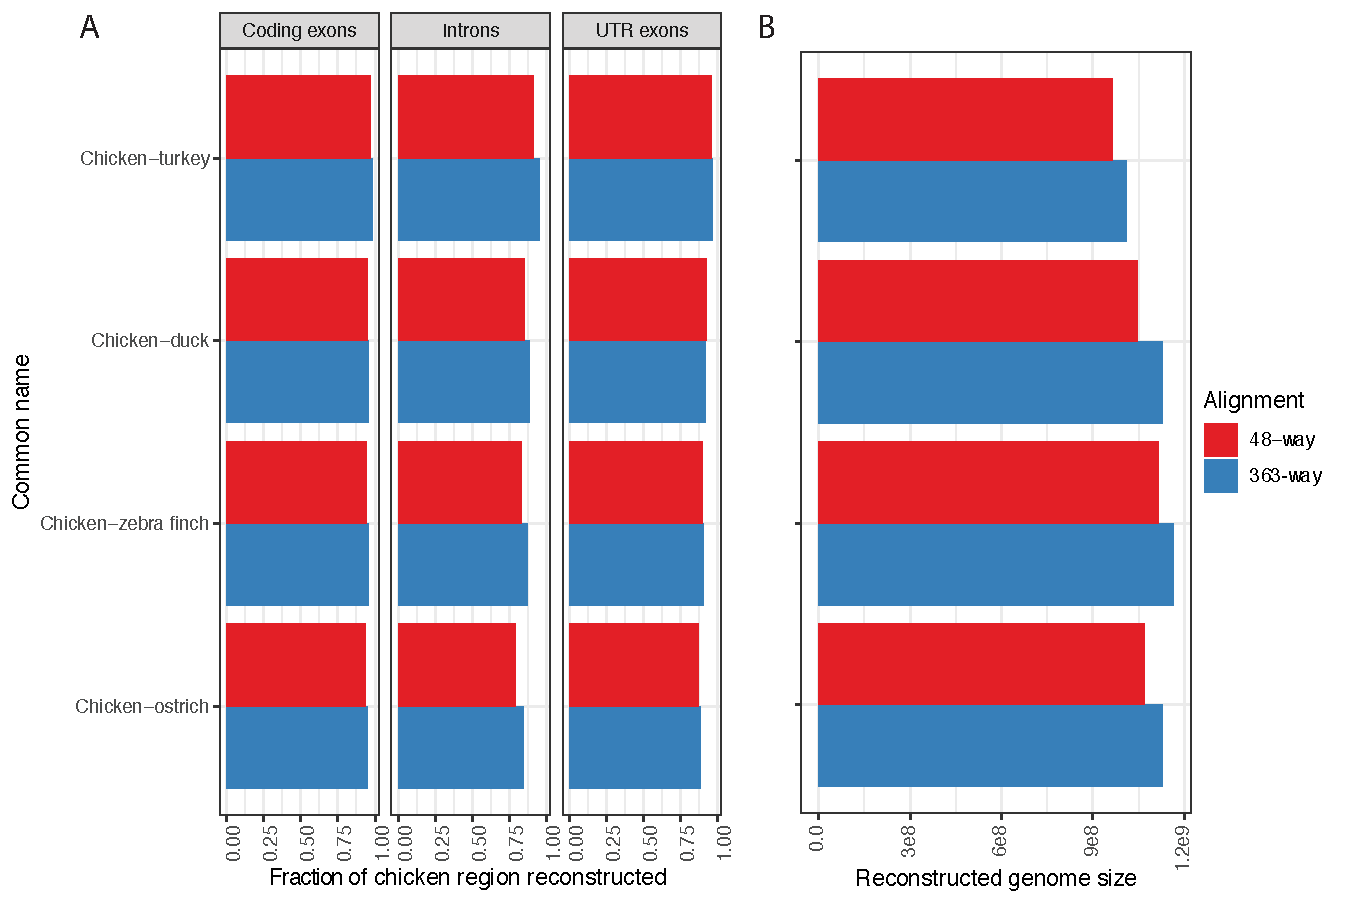
\includegraphics[width=\textwidth]{363wayvs48wayancestorscombined.pdf}
    \caption{Comparison of ancestors at the same position in the tree in a large (363-species, labeled as "363-way") and smaller (48-species, labeled as "48-way") alignment of bird genomes. A: The fraction of various types of chicken regions mappable to each ancestor within each alignment. B: The total size of each ancestral assembly within each alignment.}
    \label{fig:birdAncestorComparison} 
\end{figure}



\begin{table}
\begin{center}
\begin{tabular}{l|l}
Alignment & URL \\
\midrule
With improved filtering & \url{https://alignment-output.s3.amazonaws.com/10plusway-mapq.hal} \\
Without improved filtering & \url{https://alignment-output.s3.amazonaws.com/10plusway-master.hal} \\
\end{tabular}
\caption{Alignments compared in the paralogy-filtering evaluation.}\label{tab:mapqHals}
\end{center}
\end{table}

\begin{table}
\begin{center}
\begin{tabular}{l|l}
Genome & UCSC assembly version \\
\midrule
Tree shrew & tupChi1 \\
Kangaroo rat & dipOrd1 \\
Human & hg38 \\
Chimp & panTro6 \\
Rhesus & rheMac8 \\
Mouse & mm10 \\
Rat & rn6 \\
Dog & canFam3 \\
Cat & felCat8 \\
Pig & susScr11 \\
Cow & bosTau8 \\
Horse & equCab3 \\
Elephant & loxAfr3 \\
\end{tabular}
\caption{Assemblies used in the paralogy-filtering evaluation.}\label{tab:mapqAssemblies}
\end{center}
\end{table}


\begin{figure}
\begin{center}
\includegraphics[width=\textwidth]{region_specific_aligned_pair_breakdown.pdf}
\caption{Aligned pairs shared within specific regions (defined on the human reference) between several pairs of alignments. For Cactus alignments, duplicates have been removed for better comparison against the single-copy net alignments.}\label{fig:regionSpecificJaccards}
\end{center}
\end{figure}

\begin{figure}
\begin{center}
\includegraphics[width=0.5\textwidth]{rm_ancestor_count.pdf}
\caption[Number of L1PA6 elements within ancestral genomes]{Number of L1PA6 elements within ancestral genomes.}\label{fig:rmAncestorCount}
\end{center}
\end{figure}

\begin{figure}
\begin{center}
\includegraphics[width=0.5\textwidth]{rc_vs_no_rc.pdf}
\caption{Coverage (on the human genome) from alignments with and without removing recoverable chains after the CAF process. While the coverage is increased overall across all genomes when removing recoverable chains, the increase is relatively larger in more distant species.}\label{fig:rc_vs_no_rc}
\end{center}
\end{figure}

%%% Gene/transcript analysis

\clearpage
\begin{table}[!htb]
\begin{center}
\begin{tabular}{l|r|r|r|r}
\multicolumn{1}{c}{} & \multicolumn{4}{c}{Human to chicken} \\
\cmidrule{2-5}
Category                     & \textit{BLATX} & \textit{TBLASTX} & \textit{LASTZ} & \textit{Cactus} \\
\midrule
Source transcripts           & 84,001         & 84,001           & 84,001         & 84,001          \\
Mapped                       & 58,574         & 67,197           & 56,335         & 61,925          \\
Rate mapped                  & 0.70           & 0.80             & 0.67           & 0.74            \\
Multi-mapped                 & 9,605          & 34,573           & 1,037          & 1,634            \\
Rate multi-mapped            & 0.16           & 0.51             & 0.02           & 0.03            \\
Mean base mapping rate       & 0.33           & 0.33             & 0.44           & 0.42            \\
Median base mapping rate     & 0.32           & 0.33             & 0.48           & 0.43            \\
Mean CDS base mapping rate   & 0.50           & 0.48             & 0.60           & 0.60            \\
Median CDS base mapping rate & 0.60           & 0.56             & 0.85           & 0.79            \\
\end{tabular}
\caption{Comparison of mapping protein-coding transcripts from human to chicken
  using four alignment and mapping methods (described in \secref{sec:transcriptMappingProtocol}).  Human source
  transcripts are from GENCODE V34.
  The multi-mapped rate is computed for those source transcripts that
  have any mappings.  The base mapping rates are computed for the single best
  mapping of each mapped transcript.  
  The best mapping is defined as the mapping with the highest average of the number of bases mapped across (i) the entire transcript and (ii) just the CDS portion.
}\label{tab:humanChickenTranscriptMappingStats}
\end{center}
\end{table}

\begin{table}[!htb]
\begin{center}
\begin{tabular}{l|r|r|r|r|r|r|r}
Method           & source & mRNAs   & align   & mean  & median & mean    & median  \\
                 & mRNAs  & aligned & count   & ident & ident  & aligned & aligned \\
\midrule                           
\textit{BLATX}   &  84,001 & 58,574  & 71,691  & 0.77  & 0.76   & 0.45    & 0.42    \\
\textit{TBLASTX} &  84,001 & 67,197  & 137,270 & 0.66  & 0.65   & 0.34    & 0.31    \\
\textit{LASTZ}   &  84,001 & 56,335  & 57,496  & 0.74  & 0.74   & 0.66    & 0.68    \\
\textit{Cactus}  &  84,001 & 61,925  & 63,607  & 0.75  & 0.76   & 0.56    & 0.56    \\
\end{tabular}
\caption{Transcript alignment statistics mapping from human to chicken (described in \secref{sec:transcriptMappingProtocol}).  For each alignment method, this shows the
  number of mRNAs that were aligned (mRNAs aligned) and the total number of
  alignments of those mRNA (align count), along with the mean and median of
  the nucleotide identity and of the fraction of the mRNAs nucleotides that
  aligned.  }\label{tab:humanChickenTranscriptAlignStats}
\end{center}
\end{table}

\begin{table}[!htb]
\begin{center}
\begin{tabular}{l|r|r|r|r|r|r|r}
Method           & source & mRNAs   & align   & mean  & median & mean    & median  \\
                 & mRNAs  & aligned & count   & ident & ident  & aligned & aligned \\
\midrule                           
\textit{BLATX}   &  19,695 & 12,102 & 15,619  & 0.74  & 0.75  & 0.36  & 0.32 \\
\textit{TBLASTX} &  19,695 & 13,968 & 29,011  & 0.63  & 0.62  & 0.30  & 0.27 \\
\textit{LASTZ}   &  19,695 & 11,935 & 12,317  & 0.72  & 0.72  & 0.56  & 0.55 \\
\textit{Cactus}  &  19,695 & 12,971 & 13,227  & 0.74  & 0.74  & 0.46  & 0.43 \\
\end{tabular}
\caption{Gene alignment statistics mapping from human to chicken (described in \secref{sec:transcriptMappingProtocol}).  Here gene coordinates are defined by the longest single transcript per gene.  For each method, this shows the
  number of mRNAs that were aligned (mRNAs aligned) and the total number of
  alignments of those mRNA (align count), along with the mean and median of
  the nucleotide identity and of the fraction of the mRNAs nucleotides that
  aligned.  }\label{tab:humanChickenGeneAlignStats}
\end{center}
\end{table}

\begin{table}[!htb]
  % from alignFoolsGoldRepr dir
\begin{center}
\begin{tabular}{l|r|r|r|r|r|r|r|r}
\multicolumn{1}{c}{} & \multicolumn{4}{c|}{Gene Counts} & \multicolumn{4}{c}{CDS Base Counts} \\
\cmidrule{2-5} \cmidrule{6-9}
Category         & \multicolumn{2}{c|}{\textit{LASTZ}} & \multicolumn{2}{c|}{\textit{Cactus}}
                 & \multicolumn{2}{c|}{\textit{LASTZ}} & \multicolumn{2}{c}{\textit{Cactus}} \\
                 & count  & rate & count  & rate   & count  & rate & count  & rate   \\
  \midrule
source           & 19,695 & 1.00 & 19,695 & 1.00   & 34,356,456 & 1.00 & 34,356,456 & 1.00 \\
missing          & 3,485  & 0.18 & 3,429  & 0.17   & 4,141,477  & 0.12 & 3,967,426  & 0.12 \\
unmapped         & 4,110  & 0.21 & 2,991  & 0.15   & 6,052,342  & 0.18 & 4,083,397  & 0.12 \\
mapped hit       & 10,832 & 0.55 & 11,758 & 0.60   & 15,696,629 & 0.46 & 15,732,865 & 0.46 \\
mapped miss      & 194    & 0.01 & 387    & 0.02   & 7,499,854  & 0.22 & 9,661,280  & 0.28 \\
mapped only      & 1,074  & 0.05 & 1,130  & 0.06   & 966,154    & 0.03 & 911,488    & 0.03 \\
\end{tabular}
\caption{ % Overview
Comparison of each of the \textit{LASTZ} and \textit{Cactus} alignments to the union of the \textit{BLATX} and
  \textit{TBLASTX} translated alignments.  This analysis implicitly uses the union of the translated
  alignments as a proxy to a truth set to compare the non-translated methods.  
  % Gene set
  Human coding sequences from GENCODE V34 are used, picking the coding sequence from the longest transcript per gene to define a minimally overlapping set.
  % Multi-mapping
  To account for human bases which map to multiple bases in chicken (which occurs frequently for the translated alignment methods that include very distant, fragmented, paralogous alignments, but much less often for the non-translated methods), 
  when per CDS there is either or both multiple translated alignments or multiple non-translated alignments, we pick the pair of mappings (one translated, one from the non-translated method) with highest pairwise Jaccard similarity. Base level counts are then reported for this pairing of the CDS.  
  %The gene CDS representative transcript sets are used.  The single-best overlappingbtarget gene is used to compute the overlap for a giving gene mapping. 
  %When there are multiple mapped genes, the one with the best target overlap is used.  When there is no overlapping target genes, the mapped gene with the most mapped bases is used.
  % Genes / bases
  We report numbers in terms of genes and individual human coding bases. %% How do we define 
  % Source
  The \textit{source} row is the total number of human genes/coding bases.  
  % Missing
  The \textit{missing} counts are the number of human genes/coding bases that were not mapped by either the untranslated method (\textit{Cactus} or \textit{LASTZ}) or the one of the translated alignment methods.  
  % Unmapped
  The \textit{unmapped} are cases where there are translated alignments and no untranslated alignment.  
  % Mapped hit
  The \textit{mapped hit} are cases
  where the untranslated alignment is the same as a
  translated alignment.  
  % Mapped miss
  With \textit{mapped miss}, the untranslated alignments do
  not overlap any of the translated alignments. 
  % Mapped only
  The \textit{mapped only} are
  counts of genes/bases that are only aligned by the untranslated aligner.
  }\label{tab:humanGeneCdsToAlignedCmp}
\end{center}
\end{table}

\begin{figure}
\begin{center}
\includegraphics[width=\textwidth]{transcript_cds_human_to_chicken_pairwise_jaccard_distributions.pdf}
\caption{Distribution of Jaccard similarities between each pair of aligners for the mRNA and coding regions of each human transcript mapped to the chicken genome (details of mapping described in \secref{sec:transcriptMappingProtocol}). Where one or both aligners produces multiple mappings per transcript we pick the pair of mappings (one from each mapper) with highest overlap. If one or both methods method didn't produce an
alignment, a Jaccard index of 0.0 is assigned.\label{fig:transcriptCDSJaccards}}
\end{center}
\end{figure}

\begin{figure}
\begin{center}
\includegraphics[width=\textwidth]{gene_cds_human_to_chicken_pairwise_jaccard_distributions.pdf}
\caption{Distribution of Jaccard similarities between each pair of aligners for the mRNA and coding regions of each human of each human gene mapped to the chicken genome (details of mapping described in \secref{sec:transcriptMappingProtocol}). Where one or both aligners produces multiple mappings per gene we pick the pair of mappings (one from each mapper) with highest overlap. If one or both methods didn't produce an
alignment, a Jaccard index of 0.0 is assigned. Here gene coordinates are defined by the longest single mRNA or CDS per gene.\label{fig:geneCDSJaccards}}
\end{center}
\end{figure}



\begin{table}[!htb]
\begin{center}
\begin{tabular}{l|l|r|r|r|r}
\multicolumn{2}{c}{}               &  \multicolumn{2}{c|}{Transcripts} & \multicolumn{2}{c}{Genes} \\
\multicolumn{2}{c}{}               & \multicolumn{2}{c|}{to chicken}& \multicolumn{2}{c}{to chicken} \\
\cmidrule{3-4}\cmidrule{5-6} 
\multicolumn{2}{c}{Methods}         & mRNA & CDS   & mRNA & CDS  \\
\midrule
\textit{BLATX}    & \textit{TBLASTX} & 0.41 & 0.42 & 0.34 &  0.37 \\
\textit{BLATX}    & \textit{LASTZ}   & 0.39 & 0.45 & 0.30 &  0.38 \\
\textit{BLATX}    & \textit{Cactus}  & 0.43 & 0.46 & 0.34 &  0.40 \\
\textit{TBLASTX}  & \textit{LASTZ}   & 0.33 & 0.37 & 0.26 &  0.32 \\
\textit{TBLASTX}  & \textit{Cactus}  & 0.37 & 0.39 & 0.30 &  0.34 \\
\textit{LASTZ}    & \textit{Cactus}  & 0.50 & 0.54 & 0.41 &  0.47 \\
\end{tabular}
\caption{Similarity of mapping protein-coding transcripts and genes between human and
chicken using the four alignment and mapping methods (details of mapping described in \ref{sec:transcriptMappingProtocol}).  The metric is the
mean Jaccard index computed at the base-level of individual
transcripts.  Where one or both aligners produces multiple mappings per transcript we pick the pair of mappings (one from each mapper) with highest overlap.  If one or both methods method didn't produce an
alignment, a Jaccard index of 0.0 is assigned.
}\label{tab:humanChickenTranscriptMappingMethodSim}
\end{center}
\end{table}



\begin{table}[!htb]
\begin{center}
\begin{tabular}{l|r|r|r|r}
\multicolumn{1}{c}{} &  \multicolumn{2}{c|}{Transcripts} & \multicolumn{2}{c}{Genes} \\
\cmidrule{2-3}\cmidrule{4-5}
Method           & mRNA & CDS   & mRNA  & CDS \\
\midrule
\textit{BLATX}   & 0.34 &  0.47 &  0.57 &  0.42 \\
\textit{TBLASTX} & 0.24 &  0.32 &  0.41 &  0.31 \\
\textit{LASTZ}   & 0.43 &  0.58 &  0.63 &  0.56 \\
\textit{Cactus}  & 0.38 &  0.53 &  0.64 &  0.51 \\
\end{tabular}
\caption{
The Jaccard index similarity metric of human protein-coding transcript and gene mappings to the
native chicken transcript annotations for the four alignment methods
For each source that was mapped, we pick the target native annotation
with the highest base-level Jaccard index to any of the source
transcript's mappings as the candidate ortholog.  This table reports the
mean Jaccard index for each mapped source transcript and the chosen target
transcript.  The preliminary state of the chicken annotation as compared to
human limits the value of making absolute interpretations of the mappings'
correctness.  In particular, this analysis doesn't account for alignment
to paralogous genes.
However, it provides a useful, if limited, relative comparison.  Due to this
asymmetry in the sets (chicken has just 13,391 transcripts)
and not using independent ortholog assignment, we only
consider those alignments that actually overlap, not the non-overlapping
or non-mapping annotations.  This type of in depth ortholog comparison would
be of great value, however it is beyond the scope of this paper.
}\label{tab:humanChickenTranscriptNativeSim}
\end{center}
\end{table}

\bibliographystyle{plain}
\bibliography{references}
\end{document}
